\section{Metric Classes}
Conversion of the Workload theory into quantifiable measurements necesitated the creation of workload metric classes. See figure 4. In the interest of finding areas to consolidate actors we left off measuring team workload. Given that cognitive workload describes the difficulties presented by managing resources such as memory and inputs we named that metric class resource. Algorithmic workload anaylzes the difficulties presented by decisions giving rise to the decision metrics.


\begin{figure}[h]
\center
\setlength{\abovecaptionskip}{1mm}
\setlength{\belowcaptionskip}{1mm}
\setlength{\textfloatsep}{1mm}
\setlength{\floatsep}{1mm}
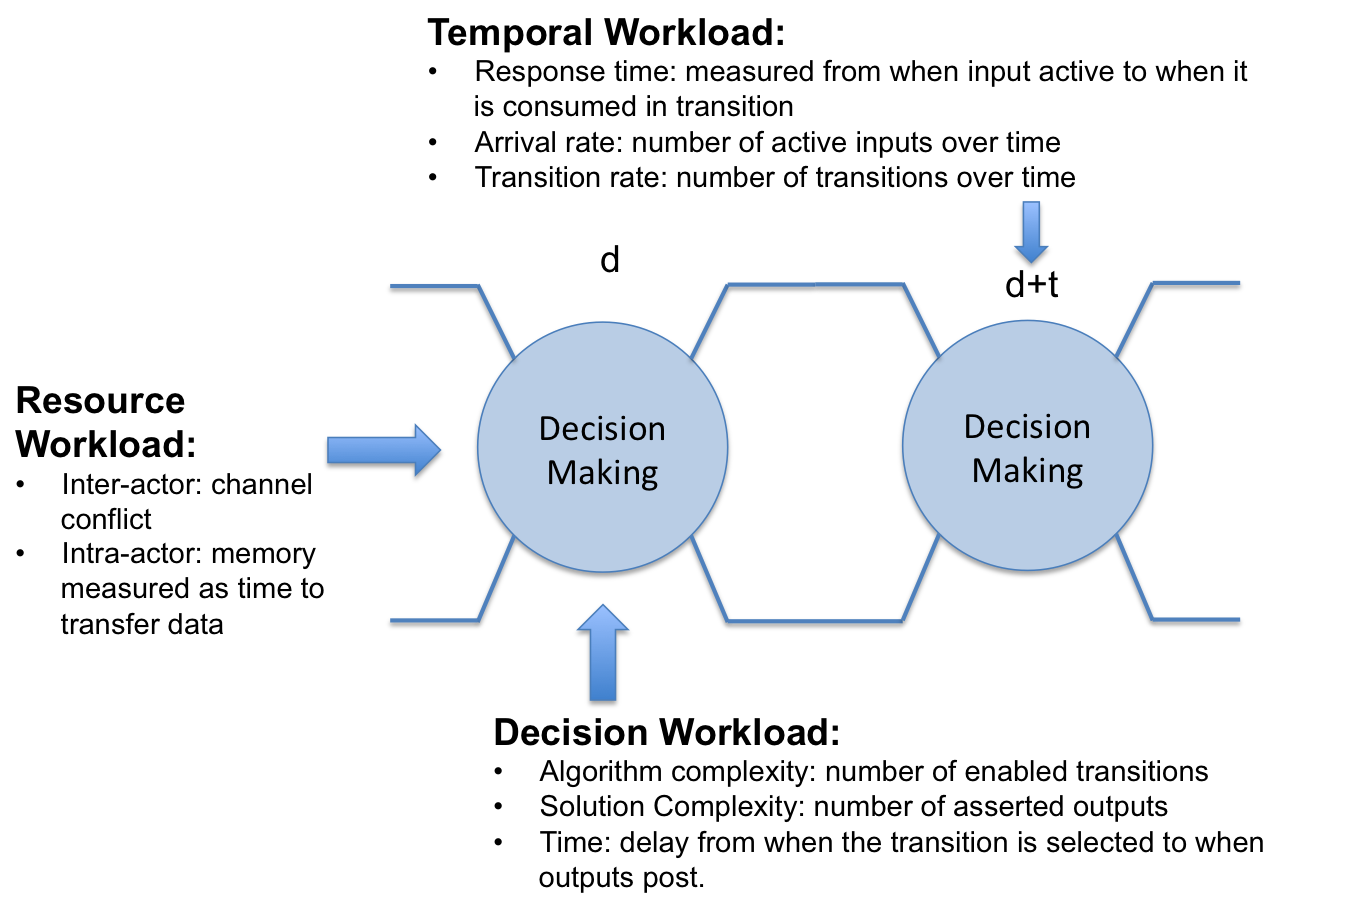
\includegraphics[height=2.5in]{WorkloadMetrics.png}
\caption{Workload in the model}
\label{fig:WorkloadMetrics}
\end{figure}

\subsection{Resource Metrics}
Cognitive workload is separated into both inter-actor communication and intra-actor memory analysis. We implemented a listener that recorded memory accesses to handle the intra-actor workload generated. The second listener built into the modeling environment records all channel reads. By using these two listeners we gained the ability to maintain an accurate view of how the cognitive workload flucuates over time.

\subsection{Temporal Metrics}
The model lent itself to measuring temporal workload using three separate metrics. The op-tempo is measured by recording how many transitions occur over a course of the simulation. Tracking the rate at which inputs become active gives an accurate reflection for the arrival rate of data. The response time is calculated by measuring the time from when an input goes active to the point when it is read by the actor.

\subsection{Decision Metrics}
Algorithmic Workload can be broken down into the timing, the complexity of the algorithm, and the complexity of the solution. The timing is calculated by measuring the time when a transition is chosen till the outputs are posted. The point when the outputs go high represents the time when that task is complete and the actor has moved on to her next task. In this fashion we meausure the time it takes to execute a given task. By counting the number of possible transitions we can track the number of choices the actor has and therefore measure the algorithmic complexity. The solution complexity is analyzed by counting the number of outputs a transition activates. This last measurement isn't very precise since some tasks are more complex than others despite requiring the same number of actions. The level of abstraction does however give us sufficient accuracy to aid in our workload predictions while keeping our metrics at a managable simplicity.